% Auto-generated by `python new.py summarize` on 2026-06-10T10:36:21.
% Folder: experiments/2026-06-10_decision_Qwen2.5-0.5B-Instruct_p5_fwd/
% Paste into a beamer document. Adjust the graphicspath or paths below if compiling from a different working directory.
%
% Requires: \usepackage{graphicx}

\begin{frame}{Binary 0/1 decision-token distribution}
  \begin{center}
    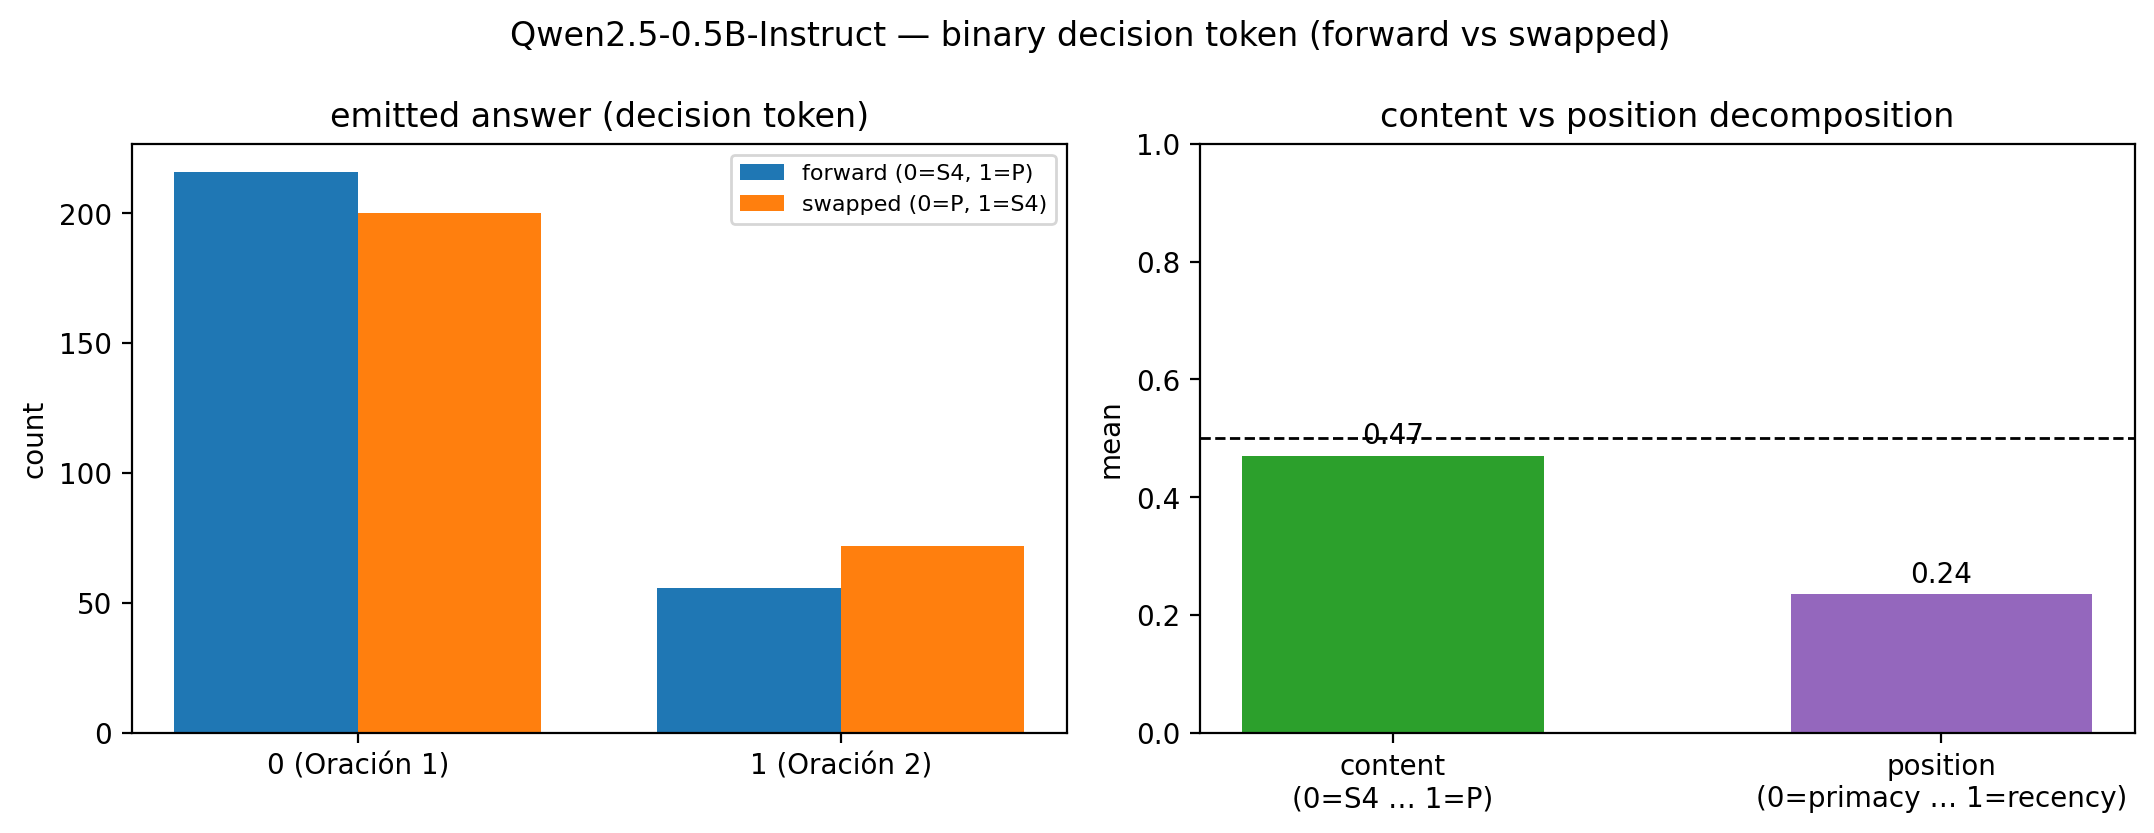
\includegraphics[width=0.95\textwidth,height=0.82\textheight,keepaspectratio]{experiments/2026-06-10_decision_Qwen2.5-0.5B-Instruct_p5_fwd/plots/decision_binary.png}
  \end{center}
\end{frame}

\begin{frame}{Binary 0/1 decision-token distribution}
  \small
  \textbf{Computation.} For paired 0/1 fwd/rev runs, count emitted answers per direction. Decompose into $\text{content} = (a + (1-b))/2$ (1 leans P) and $\text{position} = (a+b)/2$ ($>0.5$ recency, $<0.5$ primacy).
  \par\vspace{0.8em}
  \textbf{Interpretation.} Content far from $0.5$ = real S4/P preference; position far from $0.5$ = positional bias (the model picks slot 1 or slot 2 regardless of content). Large position bias with small content signal indicates behavioural noise, not preference.
\end{frame}
